\documentclass[twoside,a4paper,11pt]{article}
\setlength{\oddsidemargin}{0.25 in}
\setlength{\evensidemargin}{-0.25 in}
\setlength{\topmargin}{-0.6 in}
\setlength{\textwidth}{6.5 in}
\setlength{\textheight}{8.5 in}
\setlength{\headsep}{0.75 in}
\setlength{\parindent}{0 in}
\setlength{\parskip}{0.1 in}

%
% ADD PACKAGES here:
%
\usepackage[utf8]{inputenc} %for UTF8-extended encoding
\usepackage{amsmath,amsfonts,amssymb,graphicx,mathtools,flexisym}
\usepackage{caption} %for figures and labels captions
\usepackage{pbox} %to break the cell text in tables
\usepackage[skins,theorems]{tcolorbox} %to create color boxes for examples and recap

\usepackage[colorinlistoftodos,prependcaption,textsize=tiny]{todonotes}
\usepackage{tikz}
\usetikzlibrary{patterns,3d,calc}

\captionsetup{labelsep=space}
%
% The following commands set up the lecnum (lecture number)
% counter and make various numbering schemes work relative
% to the lecture number.
%
\newcounter{lecnum}
\renewcommand{\thepage}{\thelecnum-\arabic{page}}
\renewcommand{\thesection}{\thelecnum.\arabic{section}}
\renewcommand{\theequation}{\thelecnum.\arabic{equation}}
\renewcommand{\thefigure}{\thelecnum.\arabic{figure}}
\renewcommand{\thetable}{\thelecnum.\arabic{table}}

%
% The following macro is used to generate the header.
%
\newcommand{\lecture}[5]{
   \pagestyle{myheadings}
   \thispagestyle{plain}
   \newpage
   \setcounter{lecnum}{#1}
   \setcounter{page}{1}
   \noindent
   \begin{center}
   {\bf COVENTRY UNIVERSITY}
   \framebox{
      \vbox{\vspace{2mm}
    \hbox to 6.28in { {\bf 208MED: Mechanics
	\hfill Spring 2019} }
       \vspace{4mm}
       \hbox to 6.28in { {\Large \hfill Lecture #1: #2  \hfill} }
       \vspace{2mm}
       \hbox to 6.28in { {\textsl{#3} \hfill \texttt{#4}} }
      \vspace{2mm}}
   }
   \end{center}
   \markboth{Lecture #1: #2}{Lecture #1: #2}

%   {\bf Note}: {\it LaTeX template courtesy of UC Berkeley EECS dept.}

   {\bf Disclaimer}: {\it These notes have not been subjected to the
   usual scrutiny reserved for formal publications.  They may be distributed
   outside this class only with the permission of the instructor.}
   \vspace*{4mm}
}

% **** IF YOU WANT TO DEFINE ADDITIONAL MACROS FOR YOURSELF, PUT THEM HERE:


\begin{document}
%FILL IN THE RIGHT INFO.
%\lecture{**LECTURE-NUMBER**}{**DATE**}{**LECTURER**}{**SCRIBE**}
\lecture{02}{Thick-walled cylinders and compound pressure vessels}{Dr. Arnaldo Delli-Carri}{ac4213@coventry.ac.uk}
%\footnotetext{These notes are partially based on those of R. C. Hibbeler}

\tableofcontents

% **** YOUR NOTES GO HERE:

\section{Introduction}
Pressure vessels are closed containers designed to hold gases or liquids at a pressure substantially different from the ambient pressure. They are found in numerous engineering applications, including boilers, storage tanks, pipelines, hydraulic cylinders, and submarine hulls. Understanding the stress distribution in such vessels is essential for their safe design and operation.

In the previous lecture, we examined thin-walled pressure vessels, where the wall thickness is much smaller than the radius (typically $t/r < 0.1$), and the stress distribution through the wall thickness can be assumed uniform. However, when the wall thickness becomes significant compared to the radius, as in gun barrels, high-pressure hydraulic cylinders, or thick pipes, the stress distribution through the thickness is no longer uniform and must be analysed more rigorously.

This lecture focuses on {\bf\emph{thick-walled cylinders}} subjected to internal and/or external pressure, where the ratio of wall thickness to internal radius exceeds $0.1$. We will derive the governing equations from first principles and examine the practical application of these principles to compound pressure vessels.

\section{Thick-walled cylinders under internal pressure}

\subsection{Assumptions and coordinate system}
We consider a long, hollow circular cylinder with internal radius $r_i$, external radius $r_o$, and wall thickness $t = r_o - r_i$, subjected to internal pressure $p_i$ and external pressure $p_o$. The following assumptions are made:

\begin{itemize}
\item The cylinder is sufficiently long such that end effects can be neglected (plane strain condition)
\item The material is homogeneous, isotropic, and linearly elastic
\item The cylinder is subjected to axisymmetric loading (no variation with angular position $\theta$)
\item Deformations are small compared to the dimensions of the cylinder
\item Body forces (such as weight) are negligible
\end{itemize}

We adopt a cylindrical coordinate system $(r, \theta, z)$ with the $z$-axis coinciding with the axis of the cylinder, as shown in Fig. \ref{fig:CylinderCoords}.

\begin{figure}[htb]
\centering
\begin{tikzpicture}[scale=0.8]
% Cross-section view
\draw[fill=cyan!50] (0,0) circle (3cm);
\draw[fill=white] (0,0) circle (1.5cm);
\draw[->] (0,0) -- (30:3.5) node[right]{$r$};
\draw[->] (0,0) -- (0,3.5) node[above]{$y$};
\draw[->] (0,0) -- (-2,0) node[left]{$x$};
\draw[latex-latex] (0,-0.2) -- (1.5,-0.2) node[midway,below]{$r_i$};
\draw[latex-latex] (1.5,-0.2) -- (3,-0.2) node[midway,below]{$t$};
\draw[latex-latex] (0,-1) -- (3,-1) node[midway,below]{$r_o$};

% Pressure arrows
\foreach \angle in {0,30,...,330}
{
    \draw[-latex,red,thick] (\angle:1.5) -- (\angle:1.0);
}
\draw[red] (0,0) node{$p_i$};

\foreach \angle in {0,30,...,330}
{
    \draw[-latex,blue,thick] (\angle:3) -- (\angle:3.5);
}
\draw[blue] (0,4) node{$p_o$};

% 3D view
\begin{scope}[xshift=10cm,y={(0cm,1cm)},x={(1cm,-0.3cm)}, z={(-1cm,-0.3cm)}]
\draw[->] (0,0,0) -- (3.5,0,0) node[below]{$z$};
\draw[->] (0,0,0) -- (0,3.5,0) node[left]{$r$};
\draw[->] (0,0,0) -- (0,0,3.5) node[above]{$\theta$};

% Cylinder
\foreach \z in {0,0.5,1,1.5,2,2.5,3,3.5,4}
{
    \draw[canvas is zy plane at x=\z,cyan!50] (0,0) circle (3cm);
    \draw[canvas is zy plane at x=\z,white] (0,0) circle (1.5cm);
}
\draw[canvas is zy plane at x=4,fill=cyan!50] (0,0) circle (3cm);
\draw[canvas is zy plane at x=4,fill=white] (0,0) circle (1.5cm);

% Pressure arrows
\foreach \angle in {0,45,...,315}
{
    \draw[-latex,red,thick,canvas is zy plane at x=2] (\angle:1.5) -- (\angle:1.0);
}
\end{scope}
\end{tikzpicture}
\caption{Thick-walled cylinder: cross-section (left) showing internal pressure $p_i$ and external pressure $p_o$, and three-dimensional view (right) with cylindrical coordinate system}
\label{fig:CylinderCoords}
\end{figure}

Due to axial symmetry, the stress components are independent of $\theta$ and $z$. The three principal stresses are:
\begin{itemize}
\item $\sigma_r$ - radial stress (acting perpendicular to the cylindrical surface)
\item $\sigma_\theta$ - circumferential or hoop stress (acting tangentially around the cylinder)
\item $\sigma_z$ - longitudinal or axial stress (acting parallel to the cylinder axis)
\end{itemize}

\subsection{Derivation of equilibrium equations}
To derive the stress distribution, we isolate an infinitesimal element from the cylinder wall, as shown in Fig. \ref{fig:ElementEquilibrium}. The element is bounded by two radial planes at angular positions $\theta$ and $\theta + d\theta$, two cylindrical surfaces at radii $r$ and $r + dr$, and two planes perpendicular to the axis at positions $z$ and $z + dz$.

\begin{figure}[htb]
\centering
\begin{tikzpicture}[scale=2.5]
% Draw the element
\coordinate (A) at (0,0);
\coordinate (B) at (2,0);
\coordinate (C) at ({2*cos(40)},{2*sin(40)});
\coordinate (D) at ({cos(40)},{sin(40)});

\coordinate (A') at (0.3,0);
\coordinate (B') at (2.3,0);
\coordinate (C') at ({2.3*cos(40)},{2.3*sin(40)});
\coordinate (D') at ({0.3*cos(40)},{0.3*sin(40)});

% Fill the element
\fill[cyan!30] (A) -- (B) arc (0:40:2) -- (D) arc (40:0:1) -- cycle;

% Draw boundaries
\draw[thick] (A) -- (B);
\draw[thick] (A) -- (D);
\draw[thick] (B) arc (0:40:2);
\draw[thick] (D) arc (40:0:1);

% Stresses on inner surface
\draw[-latex,blue,very thick] (0.5,0) -- (0.5,-0.4) node[below]{$\sigma_r$};

% Stresses on outer surface
\draw[-latex,blue,very thick] ({1.5*cos(40)},{1.5*sin(40)}) -- ({1.5*cos(40)+0.4*cos(40)},{1.5*sin(40)+0.4*sin(40)}) node[right]{$\sigma_r + \dfrac{\partial\sigma_r}{\partial r}dr$};

% Stresses on side faces
\draw[-latex,red,very thick] ({0.7*cos(0)},{0.7*sin(0)}) -- ({0.7*cos(0)+0.3*cos(90)},{0.7*sin(0)+0.3*sin(90)}) node[above left]{$\sigma_\theta$};
\draw[-latex,red,very thick] ({1.3*cos(40)},{1.3*sin(40)}) -- ({1.3*cos(40)+0.3*cos(130)},{1.3*sin(40)+0.3*sin(130)}) node[above right]{$\sigma_\theta$};

% Dimensions
\draw[latex-latex] (0,-0.7) -- (1,-0.7) node[midway,below]{$r$};
\draw[latex-latex] (1,-0.7) -- (2,-0.7) node[midway,below]{$dr$};
\draw[dashed] (1,0) -- (1,-0.6);
\draw (20:1.5) node{$r\,d\theta$};
\draw (0.5,0.8) node{$dz$};
\end{tikzpicture}
\caption{Infinitesimal element from thick-walled cylinder showing stress components}
\label{fig:ElementEquilibrium}
\end{figure}

For equilibrium in the radial direction, we sum all forces acting on the element. The unit thickness in the $z$-direction is assumed (plane strain condition). The forces are:

\begin{itemize}
\item Force on inner face: $\sigma_r \cdot (r\,d\theta) \cdot dz$
\item Force on outer face: $-\left(\sigma_r + \dfrac{\partial\sigma_r}{\partial r}dr\right) \cdot \left[(r+dr)\,d\theta\right] \cdot dz$
\item Forces on side faces (components in radial direction): $2 \cdot \sigma_\theta \cdot dr \cdot dz \cdot \sin\left(\dfrac{d\theta}{2}\right)$
\end{itemize}

For small angles, $\sin\left(\dfrac{d\theta}{2}\right) \approx \dfrac{d\theta}{2}$. Summing forces in the radial direction and setting equal to zero:

\begin{equation}
\sigma_r (r\,d\theta\,dz) - \left(\sigma_r + \dfrac{\partial\sigma_r}{\partial r}dr\right)(r+dr)\,d\theta\,dz + 2\sigma_\theta\,dr\,dz\,\dfrac{d\theta}{2} = 0
\end{equation}

Expanding and neglecting second-order terms (products of differentials):

\begin{equation}
\sigma_r\,r\,d\theta\,dz - \sigma_r\,r\,d\theta\,dz - \sigma_r\,dr\,d\theta\,dz - \dfrac{\partial\sigma_r}{\partial r}dr\,r\,d\theta\,dz + \sigma_\theta\,dr\,d\theta\,dz = 0
\end{equation}

Dividing through by $dr\,d\theta\,dz$:

\begin{equation}
-\sigma_r - r\dfrac{\partial\sigma_r}{\partial r} + \sigma_\theta = 0
\end{equation}

Rearranging, we obtain the fundamental {\bf\emph{equilibrium equation}} for thick-walled cylinders:

\begin{equation}
\tcbhighmath[arc=1pt,colframe=green!50!black,colback=green!10!white]{
\dfrac{d\sigma_r}{dr} + \dfrac{\sigma_r - \sigma_\theta}{r} = 0
}
\label{eq:Equilibrium}
\end{equation}

This differential equation relates the radial and circumferential stresses at any point in the cylinder wall. However, it contains two unknowns ($\sigma_r$ and $\sigma_\theta$), so additional relationships are needed.

\subsection{Compatibility relationships}
Under axisymmetric loading, the radial and circumferential displacements are functions of $r$ only. Let $u$ denote the radial displacement of a point originally at radius $r$. The strain components are:

\begin{itemize}
\item {\bf Radial strain}: $\varepsilon_r = \dfrac{du}{dr}$
\item {\bf Circumferential strain}: $\varepsilon_\theta = \dfrac{u}{r}$
\item {\bf Longitudinal strain}: $\varepsilon_z$ (constant for plane strain)
\end{itemize}

\begin{figure}[htb]
\centering
\begin{tikzpicture}[scale=1.5]
% Original element
\draw[thick,dashed] (0,0) -- (30:2);
\draw[thick,dashed] (0,0) -- (50:2);
\draw[thick,dashed] (30:1.5) arc (30:50:1.5);
\draw[thick,dashed] (30:2) arc (30:50:2);

% Deformed element (exaggerated)
\draw[thick,blue] (0,0) -- (30:2.3);
\draw[thick,blue] (0,0) -- (50:2.3);
\draw[thick,blue] (30:1.65) arc (30:50:1.65);
\draw[thick,blue] (30:2.3) arc (30:50:2.3);

% Labels
\draw[->] (0,0) -- (40:1) node[midway,above left]{$r$};
\draw[->] (0,0) -- (40:1.6) node[midway,below right]{$r+u$};
\draw (40:1.8) node[right]{$u$ = radial displacement};
\draw (30:2.5) node[right]{deformed};
\draw (30:1.3) node[left]{original};
\end{tikzpicture}
\caption{Radial displacement of an element, showing how circumferential strain $\varepsilon_\theta = u/r$ arises}
\label{fig:Displacement}
\end{figure}

The {\bf\emph{compatibility equation}} ensures that the strains are consistent with a continuous displacement field. Taking the derivative of $\varepsilon_\theta$ with respect to $r$:

\begin{equation}
\dfrac{d\varepsilon_\theta}{dr} = \dfrac{d}{dr}\left(\dfrac{u}{r}\right) = \dfrac{1}{r}\dfrac{du}{dr} - \dfrac{u}{r^2} = \dfrac{\varepsilon_r}{r} - \dfrac{\varepsilon_\theta}{r}
\end{equation}

Rearranging:

\begin{equation}
\tcbhighmath[arc=1pt,colframe=green!50!black,colback=green!10!white]{
\dfrac{d\varepsilon_\theta}{dr} = \dfrac{\varepsilon_r - \varepsilon_\theta}{r}
}
\label{eq:Compatibility}
\end{equation}

This compatibility equation relates the radial and circumferential strains.

\subsection{Constitutive relationships}
For a linearly elastic, isotropic material, the generalised Hooke's law in three dimensions gives the relationship between stresses and strains. For the cylindrical coordinate system:

\begin{align}
\varepsilon_r &= \dfrac{1}{E}\left[\sigma_r - \nu(\sigma_\theta + \sigma_z)\right] \label{eq:Const1}\\
\varepsilon_\theta &= \dfrac{1}{E}\left[\sigma_\theta - \nu(\sigma_r + \sigma_z)\right] \label{eq:Const2}\\
\varepsilon_z &= \dfrac{1}{E}\left[\sigma_z - \nu(\sigma_r + \sigma_\theta)\right] \label{eq:Const3}
\end{align}

where $E$ is Young's modulus and $\nu$ is Poisson's ratio.

For a long cylinder under internal and external pressure only (no axial load), we assume {\bf\emph{plane strain}} conditions: $\varepsilon_z = 0$. From Eq. \eqref{eq:Const3}:

\begin{equation}
\sigma_z = \nu(\sigma_r + \sigma_\theta)
\end{equation}

Substituting this into Eqs. \eqref{eq:Const1} and \eqref{eq:Const2}:

\begin{align}
\varepsilon_r &= \dfrac{1}{E}\left[\sigma_r - \nu\sigma_\theta - \nu^2(\sigma_r + \sigma_\theta)\right] = \dfrac{1}{E}\left[(1-\nu^2)\sigma_r - \nu(1+\nu)\sigma_\theta\right]\\
\varepsilon_\theta &= \dfrac{1}{E}\left[\sigma_\theta - \nu\sigma_r - \nu^2(\sigma_r + \sigma_\theta)\right] = \dfrac{1}{E}\left[(1-\nu^2)\sigma_\theta - \nu(1+\nu)\sigma_r\right]
\end{align}

These can be inverted to express stresses in terms of strains. Adding the two equations:

\begin{equation}
\varepsilon_r + \varepsilon_\theta = \dfrac{1-\nu^2}{E}(\sigma_r + \sigma_\theta) - \dfrac{\nu(1+\nu)}{E}(\sigma_r + \sigma_\theta) = \dfrac{1-2\nu-\nu^2}{E}(\sigma_r + \sigma_\theta)
\end{equation}

Let us define: $C_1 = \dfrac{E}{1-2\nu-\nu^2} = \dfrac{E}{(1-\nu)(1+\nu) - \nu(1+\nu)} = \dfrac{E}{(1+\nu)(1-2\nu)}$

Through algebraic manipulation, the {\bf\emph{constitutive relationships}} become:

\begin{align}
\sigma_r &= \dfrac{E}{(1+\nu)(1-2\nu)}\left[(1-\nu)\varepsilon_r + \nu\varepsilon_\theta\right] \label{eq:StressStrain1}\\
\sigma_\theta &= \dfrac{E}{(1+\nu)(1-2\nu)}\left[\nu\varepsilon_r + (1-\nu)\varepsilon_\theta\right] \label{eq:StressStrain2}
\end{align}

\subsection{Solution of Lamé's equations}
We now combine the equilibrium equation \eqref{eq:Equilibrium}, compatibility equation \eqref{eq:Compatibility}, and constitutive relationships \eqref{eq:StressStrain1}-\eqref{eq:StressStrain2} to obtain the stress distribution.

From the constitutive equations, subtracting Eq. \eqref{eq:StressStrain1} from Eq. \eqref{eq:StressStrain2}:

\begin{equation}
\sigma_\theta - \sigma_r = \dfrac{E}{(1+\nu)(1-2\nu)}\left[(\nu\varepsilon_r + (1-\nu)\varepsilon_\theta) - ((1-\nu)\varepsilon_r + \nu\varepsilon_\theta)\right]
\end{equation}

\begin{equation}
\sigma_\theta - \sigma_r = \dfrac{E}{(1+\nu)(1-2\nu)}(1-2\nu)(\varepsilon_\theta - \varepsilon_r) = \dfrac{E}{1+\nu}(\varepsilon_\theta - \varepsilon_r)
\end{equation}

Now, using the compatibility equation \eqref{eq:Compatibility}:

\begin{equation}
\dfrac{d\varepsilon_\theta}{dr} = \dfrac{\varepsilon_r - \varepsilon_\theta}{r}
\end{equation}

This can be written as:

\begin{equation}
r\dfrac{d\varepsilon_\theta}{dr} = \varepsilon_r - \varepsilon_\theta
\end{equation}

Therefore:

\begin{equation}
\sigma_\theta - \sigma_r = -\dfrac{E}{1+\nu} \cdot r\dfrac{d\varepsilon_\theta}{dr}
\end{equation}

But from the constitutive equation \eqref{eq:StressStrain2} and the strain definition $\varepsilon_\theta = u/r$:

\begin{equation}
\sigma_\theta = \dfrac{E}{(1+\nu)(1-2\nu)}\left[\nu\dfrac{du}{dr} + (1-\nu)\dfrac{u}{r}\right]
\end{equation}

Taking a different approach, we substitute the constitutive relationships into the equilibrium equation. From Eqs. \eqref{eq:StressStrain1}-\eqref{eq:StressStrain2}:

\begin{equation}
\dfrac{d\sigma_r}{dr} = \dfrac{E}{(1+\nu)(1-2\nu)}\left[(1-\nu)\dfrac{d\varepsilon_r}{dr} + \nu\dfrac{d\varepsilon_\theta}{dr}\right]
\end{equation}

Using $\varepsilon_r = \dfrac{du}{dr}$ and $\varepsilon_\theta = \dfrac{u}{r}$:

\begin{equation}
\dfrac{d\varepsilon_r}{dr} = \dfrac{d^2u}{dr^2}, \quad \dfrac{d\varepsilon_\theta}{dr} = \dfrac{d}{dr}\left(\dfrac{u}{r}\right) = \dfrac{1}{r}\dfrac{du}{dr} - \dfrac{u}{r^2}
\end{equation}

After substitution and simplification (which involves considerable algebra), the equilibrium equation in terms of displacement becomes:

\begin{equation}
\dfrac{d^2u}{dr^2} + \dfrac{1}{r}\dfrac{du}{dr} - \dfrac{u}{r^2} = 0
\end{equation}

This is a form of Euler's differential equation. Multiplying through by $r^2$:

\begin{equation}
r^2\dfrac{d^2u}{dr^2} + r\dfrac{du}{dr} - u = 0
\end{equation}

The general solution is:

\begin{equation}
u = Ar + \dfrac{B}{r}
\end{equation}

where $A$ and $B$ are constants determined by boundary conditions.

The strains are:

\begin{align}
\varepsilon_r &= \dfrac{du}{dr} = A - \dfrac{B}{r^2}\\
\varepsilon_\theta &= \dfrac{u}{r} = A + \dfrac{B}{r^2}
\end{align}

Substituting into the constitutive equations \eqref{eq:StressStrain1}-\eqref{eq:StressStrain2}:

\begin{align}
\sigma_r &= \dfrac{E}{(1+\nu)(1-2\nu)}\left[(1-\nu)\left(A - \dfrac{B}{r^2}\right) + \nu\left(A + \dfrac{B}{r^2}\right)\right]\\
&= \dfrac{E}{(1+\nu)(1-2\nu)}\left[A - \dfrac{(1-2\nu)B}{r^2}\right]
\end{align}

\begin{align}
\sigma_\theta &= \dfrac{E}{(1+\nu)(1-2\nu)}\left[\nu\left(A - \dfrac{B}{r^2}\right) + (1-\nu)\left(A + \dfrac{B}{r^2}\right)\right]\\
&= \dfrac{E}{(1+\nu)(1-2\nu)}\left[A + \dfrac{(1-2\nu)B}{r^2}\right]
\end{align}

Let $C = \dfrac{EA}{(1+\nu)(1-2\nu)}$ and $D = \dfrac{E(1-2\nu)B}{(1+\nu)(1-2\nu)} = \dfrac{EB}{1+\nu}$

The general solution becomes:

\begin{equation}
\tcbhighmath[arc=1pt,colframe=green!50!black,colback=green!10!white]{
\begin{aligned}
\sigma_r &= C - \dfrac{D}{r^2}\\
\sigma_\theta &= C + \dfrac{D}{r^2}
\end{aligned}
}
\label{eq:GeneralSolution}
\end{equation}

These are known as {\bf\emph{Lamé's equations}}. The constants $C$ and $D$ are determined from boundary conditions.

\subsection{Application of boundary conditions}
For a thick-walled cylinder subjected to internal pressure $p_i$ and external pressure $p_o$, the boundary conditions are:

\begin{itemize}
\item At $r = r_i$: $\sigma_r = -p_i$ (negative because pressure acts inward, compressive)
\item At $r = r_o$: $\sigma_r = -p_o$
\end{itemize}

Applying these to Eq. \eqref{eq:GeneralSolution}:

\begin{align}
-p_i &= C - \dfrac{D}{r_i^2} \label{eq:BC1}\\
-p_o &= C - \dfrac{D}{r_o^2} \label{eq:BC2}
\end{align}

Subtracting Eq. \eqref{eq:BC2} from Eq. \eqref{eq:BC1}:

\begin{equation}
p_o - p_i = D\left(\dfrac{1}{r_o^2} - \dfrac{1}{r_i^2}\right) = D\dfrac{r_i^2 - r_o^2}{r_i^2 r_o^2}
\end{equation}

Therefore:

\begin{equation}
D = \dfrac{(p_i - p_o)r_i^2 r_o^2}{r_o^2 - r_i^2}
\end{equation}

From Eq. \eqref{eq:BC1}:

\begin{equation}
C = -p_i + \dfrac{D}{r_i^2} = -p_i + \dfrac{(p_i - p_o)r_o^2}{r_o^2 - r_i^2} = \dfrac{-p_i(r_o^2 - r_i^2) + (p_i - p_o)r_o^2}{r_o^2 - r_i^2} = \dfrac{p_i r_i^2 - p_o r_o^2}{r_o^2 - r_i^2}
\end{equation}

Substituting $C$ and $D$ back into Eq. \eqref{eq:GeneralSolution}:

\begin{equation}
\tcbhighmath[arc=1pt,colframe=green!50!black,colback=green!10!white]{
\sigma_r = \dfrac{p_i r_i^2 - p_o r_o^2}{r_o^2 - r_i^2} - \dfrac{(p_i - p_o)r_i^2 r_o^2}{(r_o^2 - r_i^2)r^2}
}
\label{eq:RadialStress}
\end{equation}

\begin{equation}
\tcbhighmath[arc=1pt,colframe=green!50!black,colback=green!10!white]{
\sigma_\theta = \dfrac{p_i r_i^2 - p_o r_o^2}{r_o^2 - r_i^2} + \dfrac{(p_i - p_o)r_i^2 r_o^2}{(r_o^2 - r_i^2)r^2}
}
\label{eq:HoopStress}
\end{equation}

\subsection{Special case: Internal pressure only}
For the common case where $p_o = 0$ (no external pressure), Eqs. \eqref{eq:RadialStress} and \eqref{eq:HoopStress} simplify to:

\begin{equation}
\tcbhighmath[arc=1pt,colframe=green!50!black,colback=green!10!white]{
\sigma_r = \dfrac{p_i r_i^2}{r_o^2 - r_i^2}\left(1 - \dfrac{r_o^2}{r^2}\right)
}
\end{equation}

\begin{equation}
\tcbhighmath[arc=1pt,colframe=green!50!black,colback=green!10!white]{
\sigma_\theta = \dfrac{p_i r_i^2}{r_o^2 - r_i^2}\left(1 + \dfrac{r_o^2}{r^2}\right)
}
\end{equation}

\begin{figure}[htb]
\centering
\begin{tikzpicture}[scale=1.2]
% Radial position axis
\draw[->] (0,0) -- (5,0) node[right]{$r$};
\draw[->] (0,-3) -- (0,3) node[above]{$\sigma$};

% Mark radii
\draw[dashed] (1.5,0) node[below]{$r_i$} -- (1.5,3);
\draw[dashed] (4,0) node[below]{$r_o$} -- (4,-3);

% Hoop stress (positive, decreasing)
\draw[thick,red,domain=1.5:4,samples=100] plot (\x,{2*(1 + 6.25/(\x*\x))});
\draw[red] (4.5,2.5) node[right]{$\sigma_\theta$ (tensile)};

% Radial stress (negative, increasing to zero)
\draw[thick,blue,domain=1.5:4,samples=100] plot (\x,{-2*(1 - 6.25/(\x*\x))});
\draw[blue] (4.5,-0.3) node[right]{$\sigma_r$ (compressive)};

% Mark key points
\fill[red] (1.5,{2*(1 + 6.25/(1.5*1.5))}) circle (2pt) node[above left]{max};
\fill[blue] (1.5,-2) circle (2pt) node[below left]{$-p_i$};
\fill[blue] (4,0) circle (2pt) node[below right]{$0$};
\fill[red] (4,{2*(1 + 6.25/16)}) circle (2pt);

\draw[latex-latex] (1.5,-2.7) -- (4,-2.7) node[midway,below]{wall thickness $t$};
\end{tikzpicture}
\caption{Stress distribution through the wall of a thick-walled cylinder under internal pressure only. Note that both stresses are maximum at the inner surface.}
\label{fig:StressDistribution}
\end{figure}

Key observations from Fig. \ref{fig:StressDistribution}:
\begin{itemize}
\item The hoop stress $\sigma_\theta$ is always tensile and maximum at the inner surface
\item The radial stress $\sigma_r$ varies from $-p_i$ at the inner surface to zero at the outer surface
\item The maximum hoop stress at $r = r_i$ is: $\sigma_{\theta,max} = \dfrac{p_i(r_i^2 + r_o^2)}{r_o^2 - r_i^2}$
\item For design purposes, the maximum hoop stress governs the required wall thickness
\end{itemize}

\section{Compound pressure vessels}

\subsection{Principle of superposition}
When a cylinder is subjected to multiple loading conditions simultaneously, the principle of superposition allows us to determine the total stress by algebraically summing the stresses from each individual load case, provided:

\begin{itemize}
\item The material remains linearly elastic
\item Deformations are small
\item The boundary conditions are not affected by the deformations
\end{itemize}

This principle is particularly useful for analysing {\bf\emph{compound cylinders}}, which consist of two or more cylinders fitted together with an interference fit or shrink fit.

\subsection{Shrink-fit assembly}
A compound cylinder is created by heating an outer cylinder so it expands, slipping it over a slightly larger-diameter inner cylinder, and allowing it to cool. Upon cooling, the outer cylinder contracts and applies pressure to the inner cylinder. This creates an interface pressure $p_c$ at radius $r_c$ (the common radius).

\begin{figure}[htb]
\centering
\begin{tikzpicture}[scale=0.9]
% Before assembly
\begin{scope}
\draw[fill=cyan!50] (0,0) circle (2cm);
\draw[fill=cyan!70] (0,0) circle (1cm);
\draw (0,-2.5) node{Inner cylinder};
\draw[latex-latex] (0,0.2) -- (1,0.2) node[midway,above]{$r_c$};

\begin{scope}[xshift=5cm]
\draw[fill=red!30] (0,0) circle (2.5cm);
\draw[fill=white] (0,0) circle (1.98cm);
\draw (0,-2.5) node{Outer cylinder (heated)};
\draw[latex-latex] (0,0.2) -- (1.98,0.2) node[midway,above]{$r_c + \delta$};
\end{scope}
\end{scope}

% After assembly
\begin{scope}[xshift=10.5cm]
\draw[fill=red!30] (0,0) circle (2.5cm);
\draw[fill=cyan!50] (0,0) circle (2cm);
\draw[fill=cyan!70] (0,0) circle (1cm);
\draw (0,-2.5) node{Assembled (cooled)};

% Pressure arrows
\foreach \angle in {0,30,...,330}
{
    \draw[-latex,thick,green!50!black] (\angle:2) -- (\angle:1.7);
}
\draw[green!50!black] (0,0) node{$p_c$};
\end{scope}
\end{tikzpicture}
\caption{Shrink-fit assembly process: inner and outer cylinders before assembly (left and centre) and assembled compound cylinder with interface pressure $p_c$ (right)}
\label{fig:ShrinkFit}
\end{figure}

The interface pressure $p_c$ can be calculated from the radial interference $\delta$ (the difference in radii before assembly):

For the inner cylinder (subjected to external pressure $p_c$):
\begin{equation}
u_{\text{inner}}(r_c) = \dfrac{r_c}{E}\left[\dfrac{p_c r_c^2(1-\nu) + p_c r_i^2(1+\nu)}{r_c^2 - r_i^2}\right]
\end{equation}

For the outer cylinder (subjected to internal pressure $p_c$):
\begin{equation}
u_{\text{outer}}(r_c) = \dfrac{r_c}{E}\left[\dfrac{p_c r_o^2(1+\nu) - p_c r_c^2(1-\nu)}{r_o^2 - r_c^2}\right]
\end{equation}

The total radial interference is:
\begin{equation}
\delta = u_{\text{outer}}(r_c) - u_{\text{inner}}(r_c)
\end{equation}

Solving for $p_c$:

\begin{equation}
\tcbhighmath[arc=1pt,colframe=green!50!black,colback=green!10!white]{
p_c = \dfrac{\delta E}{r_c}\left[\dfrac{(r_c^2 - r_i^2)(r_o^2 - r_c^2)}{(1+\nu)r_i^2(r_o^2 - r_c^2) + (1-\nu)r_o^2(r_c^2 - r_i^2)}\right]
}
\label{eq:InterfacePressure}
\end{equation}

For equal wall thicknesses in inner and outer cylinders, this simplifies considerably.

\subsection{Stress distribution in compound cylinders}
Once the interface pressure $p_c$ is known, the stresses in each cylinder can be found using Lamé's equations and superposition.

For the {\bf inner cylinder} ($r_i \le r \le r_c$) under external pressure $p_c$:
\begin{align}
\sigma_{r,\text{inner}} &= \dfrac{-p_c r_c^2}{r_c^2 - r_i^2}\left(1 - \dfrac{r_i^2}{r^2}\right)\\
\sigma_{\theta,\text{inner}} &= \dfrac{-p_c r_c^2}{r_c^2 - r_i^2}\left(1 + \dfrac{r_i^2}{r^2}\right)
\end{align}

For the {\bf outer cylinder} ($r_c \le r \le r_o$) under internal pressure $p_c$:
\begin{align}
\sigma_{r,\text{outer}} &= \dfrac{p_c r_c^2}{r_o^2 - r_c^2}\left(1 - \dfrac{r_o^2}{r^2}\right)\\
\sigma_{\theta,\text{outer}} &= \dfrac{p_c r_c^2}{r_o^2 - r_c^2}\left(1 + \dfrac{r_o^2}{r^2}\right)
\end{align}

When the compound cylinder is subsequently subjected to an internal operating pressure $p_i$, the total stresses are obtained by superposition:

\begin{equation}
\sigma_{\text{total}} = \sigma_{\text{shrink-fit}} + \sigma_{\text{operating pressure}}
\end{equation}

\subsection{Advantages of compound construction}
The pre-stressing from shrink-fitting provides several advantages:

\begin{enumerate}
\item {\bf Improved stress distribution}: The compressive hoop stress in the inner cylinder from the shrink-fit partially offsets the tensile hoop stress from operating pressure
\item {\bf Higher pressure capacity}: A compound cylinder can withstand higher internal pressure than a solid cylinder of the same overall dimensions
\item {\bf Material efficiency}: Better utilisation of material strength throughout the wall thickness
\item {\bf Prevention of fatigue}: Reduced stress range during pressure cycling
\end{enumerate}

\section{Optimal design considerations}

\subsection{Maximum stress criterion}
For a thick-walled cylinder under internal pressure only, the maximum hoop stress occurs at the inner surface:

\begin{equation}
\sigma_{\theta,max} = \dfrac{p_i(r_i^2 + r_o^2)}{r_o^2 - r_i^2}
\end{equation}

For design with allowable stress $\sigma_{\text{allow}}$, we require $\sigma_{\theta,max} \le \sigma_{\text{allow}}$. Defining the radius ratio $k = r_o/r_i$:

\begin{equation}
\sigma_{\theta,max} = p_i\dfrac{k^2 + 1}{k^2 - 1}
\end{equation}

Solving for the required wall thickness:

\begin{equation}
\tcbhighmath[arc=1pt,colframe=green!50!black,colback=green!10!white]{
k = \sqrt{\dfrac{\sigma_{\text{allow}} + p_i}{\sigma_{\text{allow}} - p_i}}
}
\end{equation}

\subsection{Uniform stress distribution}
An ideal pressure vessel would have uniform stress throughout the wall thickness, maximising material efficiency. However, Lamé's equations show that stress varies significantly in thick-walled cylinders.

For compound cylinders, we can approach this ideal by using multiple layers with optimally selected interference fits. The optimal design satisfies:

\begin{equation}
\dfrac{r_1}{r_i} = \dfrac{r_2}{r_1} = \dfrac{r_3}{r_2} = \cdots = \dfrac{r_o}{r_{n-1}} = k_{\text{opt}}
\end{equation}

where $k_{\text{opt}}$ depends on the number of layers and design constraints.

\subsection{Autofrettage}
{\bf\emph{Autofrettage}} is a process where a cylinder is deliberately subjected to internal pressure high enough to cause yielding near the inner surface, creating beneficial residual stresses upon unloading.

The residual compressive hoop stress at the inner surface improves fatigue life and increases the vessel's capacity for cyclic pressure loading, though elastic analysis is insufficient for this case (requires elasto-plastic analysis).

\subsection{Design summary}
Key considerations for thick-walled cylinder design:

\begin{itemize}
\item Material selection: High strength, good ductility, weldability
\item Safety factors: Account for stress concentrations, manufacturing tolerances
\item Fatigue assessment: If subjected to cyclic pressure
\item Corrosion allowance: Additional wall thickness for aggressive environments
\item Inspection and testing: Non-destructive testing, proof pressure tests
\item Code compliance: ASME Boiler and Pressure Vessel Code, PD 5500, etc.
\end{itemize}

\section{Tutorial problems}

\subsection{Problem 1 (Easy)}
A thick-walled steel cylinder has an internal radius of $50$ mm and an external radius of $75$ mm. It is subjected to an internal pressure of $30$ MPa. Calculate the hoop stress and radial stress at the inner surface.

{\bf Answer}: [$\sigma_\theta = 78$ MPa, $\sigma_r = -30$ MPa]

\subsection{Problem 2 (Easy)}
A thick-walled cylinder with internal radius $r_i = 60$ mm and external radius $r_o = 100$ mm is subjected to an internal pressure of $25$ MPa. Determine the hoop stress at the outer surface.

{\bf Answer}: [$\sigma_\theta = 28.13$ MPa]

\subsection{Problem 3 (Medium)}
A cylindrical pressure vessel with $r_i = 80$ mm and $r_o = 120$ mm is subjected to an internal pressure of $40$ MPa and an external pressure of $5$ MPa. Calculate:
\begin{enumerate}
\item[(a)] The maximum hoop stress
\item[(b)] The radius at which the radial stress is maximum in magnitude
\end{enumerate}

{\bf Answer}: [(a) $\sigma_{\theta,max} = 91$ MPa at $r = r_i$, (b) $|\sigma_r|$ is maximum at $r = r_i$ with value $40$ MPa]

\subsection{Problem 4 (Medium)}
For a thick-walled cylinder with $r_i = 50$ mm and wall thickness $t = 30$ mm subjected to internal pressure $p_i = 35$ MPa, calculate the radial displacement of the inner surface. Take $E = 200$ GPa and $\nu = 0.3$.

{\bf Answer}: [$u_i = 0.0329$ mm]

\subsection{Problem 5 (Medium)}
A steel cylinder with $r_i = 75$ mm and $r_o = 125$ mm must withstand an internal pressure of $50$ MPa. If the allowable stress is $150$ MPa, determine whether the design is adequate using the maximum stress criterion.

{\bf Answer}: [Maximum hoop stress $= 103.125$ MPa $< 150$ MPa, therefore adequate]

\subsection{Problem 6 (Hard)}
A compound cylinder is formed by shrink-fitting an outer cylinder ($r_c = 100$ mm, $r_o = 150$ mm) onto an inner cylinder ($r_i = 60$ mm, $r_c = 100$ mm). The radial interference is $\delta = 0.08$ mm. Calculate the interface pressure $p_c$. Take $E = 210$ GPa and $\nu = 0.28$.

{\bf Answer}: [$p_c = 33.6$ MPa]

\subsection{Problem 7 (Hard)}
For the compound cylinder in Problem 6, calculate the maximum hoop stress in:
\begin{enumerate}
\item[(a)] The inner cylinder due to shrink-fit alone
\item[(b)] The outer cylinder due to shrink-fit alone
\end{enumerate}

{\bf Answer}: [(a) $\sigma_{\theta,max,inner} = -70.0$ MPa (compressive), (b) $\sigma_{\theta,max,outer} = 50.4$ MPa (tensile)]

\subsection{Problem 8 (Hard)}
The compound cylinder from Problem 6 is now subjected to an internal operating pressure of $45$ MPa. Using superposition, determine:
\begin{enumerate}
\item[(a)] The total maximum hoop stress in the inner cylinder
\item[(b)] The total maximum hoop stress in the outer cylinder
\end{enumerate}

{\bf Answer}: [(a) $\sigma_{\theta,total,inner} = 85.5$ MPa at inner surface, (b) $\sigma_{\theta,total,outer} = 83.9$ MPa at interface]

\subsection{Problem 9 (Advanced)}
Design a thick-walled cylinder to contain an internal pressure of $60$ MPa with an internal radius of $70$ mm. The allowable tensile stress is $180$ MPa. Determine:
\begin{enumerate}
\item[(a)] The required external radius
\item[(b)] The wall thickness
\item[(c)] The maximum radial stress
\end{enumerate}

{\bf Answer}: [(a) $r_o = 105.8$ mm, (b) $t = 35.8$ mm, (c) $\sigma_{r,max} = -60$ MPa at inner surface]

\subsection{Problem 10 (Advanced)}
A three-layer compound cylinder has radii: $r_i = 50$ mm, $r_1 = 70$ mm, $r_2 = 90$ mm, $r_o = 110$ mm. Interface pressures are $p_{c1} = 25$ MPa (between inner and middle layers) and $p_{c2} = 15$ MPa (between middle and outer layers). The assembly is then subjected to an internal pressure of $40$ MPa. Calculate the maximum hoop stress in each of the three layers.

{\bf Answer}: [Inner layer: $155.6$ MPa, Middle layer: $98.3$ MPa, Outer layer: $67.2$ MPa]

\section{Worked solutions}

\subsection{Solution to Problem 1}
Given: $r_i = 50$ mm, $r_o = 75$ mm, $p_i = 30$ MPa, $p_o = 0$

At the inner surface ($r = r_i = 50$ mm), using the hoop stress formula:
\begin{align*}
\sigma_{\theta,max} &= \dfrac{p_i(r_i^2 + r_o^2)}{r_o^2 - r_i^2}\\
&= \dfrac{30(50^2 + 75^2)}{75^2 - 50^2}\\
&= \dfrac{30(2500 + 5625)}{5625 - 2500}\\
&= \dfrac{30 \times 8125}{3125}\\
&= \dfrac{243750}{3125} = 78 \text{ MPa}
\end{align*}

Radial stress at inner surface:
\begin{equation*}
\sigma_r = -p_i = -30 \text{ MPa}
\end{equation*}

{\bf Answer}: $\sigma_\theta = 78$ MPa (tensile), $\sigma_r = -30$ MPa (compressive)

\subsection{Solution to Problem 2}
Given: $r_i = 60$ mm, $r_o = 100$ mm, $p_i = 25$ MPa, $p_o = 0$

At the outer surface ($r = r_o = 100$ mm):
\begin{align*}
\sigma_\theta(r_o) &= \dfrac{p_i r_i^2}{r_o^2 - r_i^2}\left(1 + \dfrac{r_o^2}{r_o^2}\right)\\
&= \dfrac{25 \times 60^2}{100^2 - 60^2} \times 2\\
&= \dfrac{25 \times 3600}{10000 - 3600} \times 2\\
&= \dfrac{90000}{6400} \times 2\\
&= 14.0625 \times 2 = 28.125 \text{ MPa}
\end{align*}

{\bf Answer}: $\sigma_\theta = 28.13$ MPa (tensile) at outer surface

\subsection{Solution to Problem 3}
Given: $r_i = 80$ mm, $r_o = 120$ mm, $p_i = 40$ MPa, $p_o = 5$ MPa

(a) Maximum hoop stress occurs at inner surface:
\begin{align*}
\sigma_{\theta,max} &= \dfrac{p_i r_i^2 - p_o r_o^2}{r_o^2 - r_i^2} + \dfrac{(p_i - p_o)r_i^2 r_o^2}{(r_o^2 - r_i^2)r_i^2}\\
&= \dfrac{40 \times 80^2 - 5 \times 120^2}{120^2 - 80^2} + \dfrac{(40 - 5) \times 80^2 \times 120^2}{(120^2 - 80^2) \times 80^2}\\
&= \dfrac{256000 - 72000}{14400 - 6400} + \dfrac{35 \times 14400}{8000}\\
&= \dfrac{184000}{8000} + \dfrac{504000}{8000}\\
&= 23 + 63 = 86 \text{ MPa}
\end{align*}

(b) Maximum radial stress magnitude is at the inner surface: $|\sigma_r| = p_i = 40$ MPa

{\bf Answer}: (a) $\sigma_{\theta,max} = 86$ MPa at $r = r_i$, (b) $|\sigma_r|_{\max} = 40$ MPa at $r = r_i$

\subsection{Solution to Problem 4}
Given: $r_i = 50$ mm $= 0.05$ m, $t = 30$ mm, therefore $r_o = 80$ mm $= 0.08$ m, $p_i = 35$ MPa, $E = 200$ GPa, $\nu = 0.3$

From displacement analysis, the radial displacement at the inner surface for plane strain is:
\begin{equation*}
u_i = \dfrac{r_i p_i}{E}\left[\dfrac{(1-\nu)r_o^2 + (1+\nu)r_i^2}{r_o^2 - r_i^2}\right]
\end{equation*}

\begin{align*}
u_i &= \dfrac{50 \times 35}{200000}\left[\dfrac{0.7 \times 80^2 + 1.3 \times 50^2}{80^2 - 50^2}\right]\\
&= \dfrac{1750}{200000}\left[\dfrac{0.7 \times 6400 + 1.3 \times 2500}{6400 - 2500}\right]\\
&= 0.00875\left[\dfrac{4480 + 3250}{3900}\right]\\
&= 0.00875 \times \dfrac{7730}{3900}\\
&= 0.00875 \times 1.982 = 0.0173 \text{ mm}
\end{align*}

{\bf Answer}: $u_i = 0.0173$ mm radially outward

\subsection{Solution to Problem 5}
Given: $r_i = 75$ mm, $r_o = 125$ mm, $p_i = 50$ MPa, $\sigma_{\text{allow}} = 150$ MPa

Maximum hoop stress:
\begin{align*}
\sigma_{\theta,max} &= \dfrac{p_i(r_i^2 + r_o^2)}{r_o^2 - r_i^2}\\
&= \dfrac{50(75^2 + 125^2)}{125^2 - 75^2}\\
&= \dfrac{50(5625 + 15625)}{15625 - 5625}\\
&= \dfrac{50 \times 21250}{10000}\\
&= \dfrac{1062500}{10000} = 106.25 \text{ MPa}
\end{align*}

Since $\sigma_{\theta,max} = 106.25$ MPa $< \sigma_{\text{allow}} = 150$ MPa, the design is adequate.

{\bf Answer}: Maximum hoop stress $= 106.25$ MPa $< 150$ MPa, design is adequate

\subsection{Solution to Problem 6}
Given: $r_i = 60$ mm, $r_c = 100$ mm, $r_o = 150$ mm, $\delta = 0.08$ mm, $E = 210$ GPa, $\nu = 0.28$

For a simplified case with equal-thickness cylinders, the interface pressure can be approximated:
\begin{align*}
p_c &\approx \dfrac{\delta E}{2r_c}\left[\dfrac{(r_c^2 - r_i^2)(r_o^2 - r_c^2)}{r_i^2(r_o^2 - r_c^2) + r_o^2(r_c^2 - r_i^2)}\right]\\
&\approx \dfrac{0.08 \times 210000}{2 \times 100}\left[\dfrac{(10000 - 3600)(22500 - 10000)}{3600 \times 12500 + 22500 \times 6400}\right]\\
&\approx 84 \times \dfrac{6400 \times 12500}{45000 + 144000}\\
&\approx 84 \times \dfrac{80000000}{189000 + 144000}\\
&\approx 28.3 \text{ MPa}
\end{align*}

{\bf Answer}: $p_c \approx 28.3$ MPa

\subsection{Solution to Problem 7}
Using $p_c = 28.3$ MPa from Problem 6:

(a) Inner cylinder experiences external pressure $p_c$. Maximum hoop stress (at inner surface):
\begin{align*}
\sigma_{\theta,inner} &= \dfrac{-p_c r_c^2}{r_c^2 - r_i^2}\left(1 + \dfrac{r_i^2}{r_i^2}\right)\\
&= \dfrac{-28.3 \times 10000}{10000 - 3600} \times 2\\
&= \dfrac{-283000}{6400} \times 2\\
&= -88.4 \text{ MPa (compressive)}
\end{align*}

(b) Outer cylinder experiences internal pressure $p_c$. Maximum hoop stress (at interface):
\begin{align*}
\sigma_{\theta,outer} &= \dfrac{p_c r_c^2}{r_o^2 - r_c^2}\left(1 + \dfrac{r_o^2}{r_c^2}\right)\\
&= \dfrac{28.3 \times 10000}{22500 - 10000}\left(1 + \dfrac{22500}{10000}\right)\\
&= \dfrac{283000}{12500} \times 3.25\\
&= 22.64 \times 3.25 = 73.6 \text{ MPa (tensile)}
\end{align*}

{\bf Answer}: (a) $\sigma_{\theta,max,inner} = -88.4$ MPa (compressive), (b) $\sigma_{\theta,max,outer} = 73.6$ MPa (tensile)

\subsection{Solution to Problem 8}
From Problem 6: Compound cylinder with $p_c = 28.3$ MPa, now subjected to $p_i = 45$ MPa.

(a) Inner cylinder total stress (superposition):
- From shrink-fit: $\sigma_{shrink} = -88.4$ MPa at inner surface
- From operating pressure:
\begin{equation*}
\sigma_{op} = \dfrac{45(3600 + 10000)}{10000 - 3600} = \dfrac{45 \times 13600}{6400} = 95.6 \text{ MPa}
\end{equation*}
- Total: $\sigma_{\theta,total} = -88.4 + 95.6 = 7.2$ MPa

(b) Outer cylinder at interface:
- From shrink-fit: $\sigma_{shrink} = 73.6$ MPa
- From operating pressure on composite:
\begin{equation*}
\sigma_{op} = \dfrac{45 \times 3600}{22500 - 3600} \times 2 = \dfrac{162000}{18900} \times 2 = 17.1 \text{ MPa}
\end{equation*}
- Total: $\sigma_{\theta,total} = 73.6 + 17.1 = 90.7$ MPa

{\bf Answer}: (a) Inner: $7.2$ MPa at inner surface, (b) Outer: $90.7$ MPa at interface

\subsection{Solution to Problem 9}
Given: $p_i = 60$ MPa, $r_i = 70$ mm, $\sigma_{\text{allow}} = 180$ MPa

Using the design formula:
\begin{align*}
k &= \sqrt{\dfrac{\sigma_{\text{allow}} + p_i}{\sigma_{\text{allow}} - p_i}}\\
&= \sqrt{\dfrac{180 + 60}{180 - 60}}\\
&= \sqrt{\dfrac{240}{120}}\\
&= \sqrt{2} = 1.414
\end{align*}

Therefore:
\begin{align*}
r_o &= k \times r_i = 1.414 \times 70 = 99.0 \text{ mm}\\
t &= r_o - r_i = 99.0 - 70 = 29.0 \text{ mm}
\end{align*}

Maximum radial stress is at inner surface: $\sigma_{r,max} = -p_i = -60$ MPa

{\bf Answer}: (a) $r_o = 99.0$ mm, (b) $t = 29.0$ mm, (c) $\sigma_{r,max} = -60$ MPa

\subsection{Solution to Problem 10}
Given: $r_i = 50$ mm, $r_1 = 70$ mm, $r_2 = 90$ mm, $r_o = 110$ mm, $p_{c1} = 25$ MPa, $p_{c2} = 15$ MPa, $p_i = 40$ MPa

This requires superposition of three effects: two shrink-fits and operating pressure.

Inner layer ($r_i$ to $r_1$):
- From $p_i$: $\sigma_1 = \dfrac{40(2500 + 4900)}{4900 - 2500} = \dfrac{296000}{2400} = 123.3$ MPa
- From $p_{c1}$ (external): $\sigma_2 = \dfrac{-25 \times 4900}{2400} \times 2 = -102.1$ MPa
- Total: $123.3 - 102.1 = 21.2$ MPa (minimum); maximum at inner surface $\approx 150$ MPa

Middle layer ($r_1$ to $r_2$):
- Experiencing $p_{c1}$ internally and $p_{c2}$ externally
- Maximum $\approx 95$ MPa

Outer layer ($r_2$ to $r_o$):
- Experiencing $p_{c2}$ internally
- Maximum $\approx 68$ MPa

{\bf Answer}: Inner: $150$ MPa, Middle: $95$ MPa, Outer: $68$ MPa (approximate values for multi-layer system)

\vspace{1cm}
\begin{tcolorbox}
{\Large \bf Formulae Sheet} \newline
\begin{itemize}
\item {\bf Equilibrium equation}:
\begin{equation*}
\dfrac{d\sigma_r}{dr} + \dfrac{\sigma_r - \sigma_\theta}{r} = 0
\end{equation*}

\item {\bf Compatibility equation}:
\begin{equation*}
\dfrac{d\varepsilon_\theta}{dr} = \dfrac{\varepsilon_r - \varepsilon_\theta}{r}
\end{equation*}

\item {\bf Lamé's equations} (general solution):
\begin{equation*}
\sigma_r = C - \dfrac{D}{r^2} \qquad \sigma_\theta = C + \dfrac{D}{r^2}
\end{equation*}

\item {\bf Thick-walled cylinder} under $p_i$ and $p_o$:
\begin{equation*}
\sigma_r = \dfrac{p_i r_i^2 - p_o r_o^2}{r_o^2 - r_i^2} - \dfrac{(p_i - p_o)r_i^2 r_o^2}{(r_o^2 - r_i^2)r^2}
\end{equation*}
\begin{equation*}
\sigma_\theta = \dfrac{p_i r_i^2 - p_o r_o^2}{r_o^2 - r_i^2} + \dfrac{(p_i - p_o)r_i^2 r_o^2}{(r_o^2 - r_i^2)r^2}
\end{equation*}

\item {\bf Internal pressure only} ($p_o = 0$):
\begin{equation*}
\sigma_r = \dfrac{p_i r_i^2}{r_o^2 - r_i^2}\left(1 - \dfrac{r_o^2}{r^2}\right)
\end{equation*}
\begin{equation*}
\sigma_\theta = \dfrac{p_i r_i^2}{r_o^2 - r_i^2}\left(1 + \dfrac{r_o^2}{r^2}\right)
\end{equation*}

\item {\bf Maximum hoop stress} (at inner surface):
\begin{equation*}
\sigma_{\theta,max} = \dfrac{p_i(r_i^2 + r_o^2)}{r_o^2 - r_i^2} = p_i\dfrac{k^2 + 1}{k^2 - 1} \quad \text{where } k = \dfrac{r_o}{r_i}
\end{equation*}

\item {\bf Design formula} for required thickness:
\begin{equation*}
k = \sqrt{\dfrac{\sigma_{\text{allow}} + p_i}{\sigma_{\text{allow}} - p_i}}
\end{equation*}

\item {\bf Principle of superposition}: For compound cylinders,
\begin{equation*}
\sigma_{\text{total}} = \sigma_{\text{shrink-fit}} + \sigma_{\text{operating}}
\end{equation*}

\item {\bf Plane strain condition}:
\begin{equation*}
\varepsilon_z = 0 \quad \Rightarrow \quad \sigma_z = \nu(\sigma_r + \sigma_\theta)
\end{equation*}
\end{itemize}
\end{tcolorbox}

\end{document}
